\capitulo{5}{Aspectos relevantes del desarrollo del proyecto}
\label{aspectos_relevantes}

En este capítulo se describen las decisiones, dificultades y mejoras más relevantes surgidas durante el desarrollo de la aplicación web. Se incluyen tanto los aspectos relacionados con la comprensión inicial del algoritmo C4.5 como las decisiones adoptadas para mejorar la utilidad didáctica, la navegación, la visualización de los árboles generados y la carga de conjuntos de datos personalizados.

\section{Preparación inicial y comprensión del algoritmo C4.5}

Al inicio del proyecto no se había cursado la asignatura de Minería de Datos, materia en la que se estudian con mayor profundidad los algoritmos de árboles de decisión, entre ellos C4.5. Por este motivo, antes de comenzar la implementación de la aplicación fue necesario realizar un trabajo previo de investigación y aprendizaje sobre el funcionamiento del algoritmo.

Esta fase inicial se centró en comprender los conceptos fundamentales necesarios para implementar C4.5, como la entropía, la ganancia de información, el \textit{split info}, el \textit{gain ratio}, la selección de umbrales para atributos numéricos y la poda del árbol. El objetivo no consistía únicamente en conocer de manera superficial el algoritmo, sino en ser capaz de explicar su funcionamiento mediante ejemplos prácticos y trasladarlo posteriormente a una herramienta didáctica.

Para ello, se consultaron fuentes especializadas relacionadas con árboles de decisión y aprendizaje automático. Además, se utilizaron herramientas de inteligencia artificial, como ChatGPT~\cite{chatgpt}, como apoyo didáctico para resolver dudas concretas, contrastar explicaciones y construir ejemplos que permitieran comprobar la comprensión del algoritmo antes de iniciar su desarrollo.

Como resultado de esta fase, se elaboró un ejemplo completo del funcionamiento de C4.5 que permitió mostrar a los tutores la comprensión alcanzada sobre el algoritmo. Este trabajo previo fue relevante para definir posteriormente la estructura de la simulación y los cálculos que debían mostrarse al usuario.

En cuanto a las tecnologías utilizadas, no fue necesario realizar un proceso de selección amplio, ya que se decidió mantener la base tecnológica empleada en la aplicación web desarrollada previamente para el algoritmo ID3 \cite{drefs2026DecisionTreeSimulator}. Esta decisión permitió conservar una experiencia de uso coherente entre ambas herramientas y aprovechar componentes, estilos y mecanismos de interacción ya utilizados en el proyecto anterior.

\section{Evolución de la explicación teórica del algoritmo}

Uno de los primeros retos del proyecto consistió en decidir cómo presentar los conceptos teóricos del algoritmo C4.5 de una forma comprensible y didáctica. Aunque la entropía ya había sido explicada en la aplicación dedicada al algoritmo ID3, C4.5 incorpora nuevos elementos que requieren una explicación específica, el \textit{split info}, el \textit{gain ratio} y el tratamiento de valores numéricos.

Inicialmente, se planteó una explicación lineal y secuencial del algoritmo. En este diseño, el usuario debía avanzar por los diferentes pasos del proceso hasta llegar a la selección del atributo o nodo correspondiente. Sin embargo, durante el desarrollo se identificó una limitación de usabilidad: si el usuario tenía dudas sobre un cálculo concreto situado al final del proceso, debía recorrer todos los pasos anteriores para localizar la explicación necesaria.

Para resolver este problema, se decidió dividir los conceptos en secciones independientes y accesibles de forma directa. De este modo, el usuario puede estudiar cada parte del algoritmo sin necesidad de seguir obligatoriamente un recorrido lineal. Esta organización permite consultar de manera individual la entropía, la ganancia de información, la información de división, la razón de ganancia o los cálculos asociados a los atributos numéricos.

Además, se consideró importante que el usuario no se limitara a consultar explicaciones estáticas. Por este motivo, se incorporó la posibilidad de introducir datos y comprobar los resultados generados por cada parte del algoritmo. No obstante, solicitar al usuario que introdujera manualmente los mismos datos en cada una de las secciones podía resultar repetitivo y poco práctico.

Como solución, se desarrolló una tabla dinámica que permite generar un conjunto de datos a partir de unas indicaciones básicas. A partir de dicha tabla, la aplicación calcula y muestra los valores necesarios para comprender cada una de las etapas del algoritmo. De este modo, el usuario puede utilizar un mismo conjunto de datos para estudiar diferentes conceptos sin tener que introducir la información repetidamente. En la figura \ref{Fig_5.1} se representa la imagen de la tabla dinámica, de la tábla ordenada y de los valores calculados.

 \begin{figure}[htbp]
     \centering
     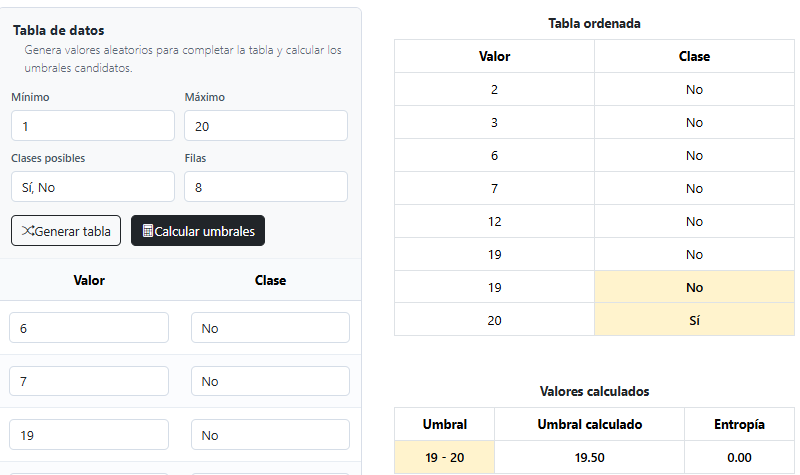
\includegraphics[width=0.75\textwidth]{img/Tabla_Dinamica_C45.png}
     \caption{Tabla dinámica para la introducción de datos y visualización de cálculos.}
     \label{Fig_5.1}
 \end{figure}

\section{Navegación contextual entre los cálculos teóricos}

Una vez definida la estructura de las secciones teóricas, se identificó una segunda dificultad relacionada con la navegación. Aunque la tabla dinámica permitía reutilizar los datos introducidos, el usuario podía seguir teniendo dudas sobre el origen de un valor concreto mostrado en una tabla de resultados.

Por ejemplo, al consultar la tabla correspondiente a la selección de un nodo, un usuario podría querer saber cómo se ha obtenido el valor de la entropía, de la ganancia de información o del \textit{gain ratio} asociado a un atributo determinado. Obligarle a buscar manualmente la sección correspondiente y volver a introducir o localizar los datos supondría una interrupción innecesaria del proceso de aprendizaje.

Para mejorar esta experiencia, se incorporaron dos mecanismos complementarios. En primer lugar, se añadieron \textit{tooltips} informativos que muestran la fórmula o el criterio utilizado para calcular determinados valores. En la figura \ref{Fig_5.1} se muestra el ejemplo del \textit{tooltip} de la tabla de valores calculados en la sección de elección de nodo. De esta manera, el usuario puede consultar la información básica sin abandonar la sección en la que se encuentra.

\begin{figure}[htbp]
     \centering
     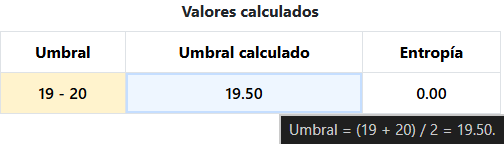
\includegraphics[width=0.75\textwidth]{img/Tooltip_Eleccion_Nodo.png}
     \caption{\textit{Tooltip} de la tabla de valores calculados en la sección de elección de nodo.}
     \label{Fig_5.2}
 \end{figure}

En segundo lugar, se implementó una navegación contextual desde las propias celdas de las tablas de resultados. Al seleccionar un valor sobre el que el usuario tiene dudas, la aplicación dirige automáticamente a la sección teórica correspondiente, conservando los datos previamente introducidos. Esta decisión permite seguir el origen de los cálculos sin tener que cargar de nuevo el conjunto de datos ni repetir las acciones realizadas anteriormente.

Con esta funcionalidad se consigue una navegación más dinámica entre los conceptos teóricos, facilitando que el usuario pueda comprender cómo se relacionan los diferentes cálculos que intervienen en el algoritmo C4.5.

\section{Diseño de la simulación de construcción del árbol C4.5}

Una vez desarrollada la parte teórica de la aplicación, se abordó la construcción de la simulación paso a paso del algoritmo C4.5. Las tecnologías utilizadas estaban condicionadas por la decisión inicial de mantener la coherencia con la aplicación desarrollada para el algoritmo ID3 \cite{drefs2026DecisionTreeSimulator}. Por tanto, la principal dificultad no residió en la selección tecnológica, sino en la organización de los elementos que debían mostrarse simultáneamente en la interfaz.

En una primera aproximación se planteó utilizar una estructura similar a la empleada en la aplicación del algoritmo ID3. Sin embargo, durante las pruebas se comprobó que esta organización no resultaba adecuada para C4.5. Incluso utilizando conjuntos de datos de tamaño similar, el algoritmo genera una cantidad mayor de información debido al cálculo de umbrales, a la evaluación de atributos numéricos y a la necesidad de mostrar tanto la ganancia de información como el \textit{gain ratio}.

Además, los árboles generados por C4.5 pueden alcanzar una mayor complejidad visual que los obtenidos mediante ID3. Por este motivo, se decidió trabajar con ejemplos de árboles de mayor tamaño durante el desarrollo. Esta decisión permitió identificar problemas de visualización, distribución de componentes y navegación antes de finalizar la aplicación.

Para adaptar la interfaz a esta complejidad, se implementaron paneles retráctiles en las principales secciones de la simulación: el panel del árbol, el panel del conjunto de datos y el panel de cálculos. De esta forma, el usuario puede ocultar temporalmente la información que no necesita consultar y ampliar el espacio disponible para los elementos que resulten relevantes en cada momento. En las figuras \ref{Fig_5.3} y \ref{Fig_5.4} se muestran los paneles retráctiles contraídos y expandidos para que visualizar la diferencia de visión del árbol en uno y en otro.

Por ejemplo, si el usuario necesita analizar la tabla de cálculos, puede reducir el espacio ocupado por el árbol o por el conjunto de datos. Del mismo modo, si desea observar la estructura del árbol con mayor claridad, puede ocultar los paneles relacionados con los cálculos. Esta decisión mejora la legibilidad de la aplicación y permite adaptar la interfaz a las necesidades del usuario durante la simulación.


\begin{figure}[htbp]
     \centering
     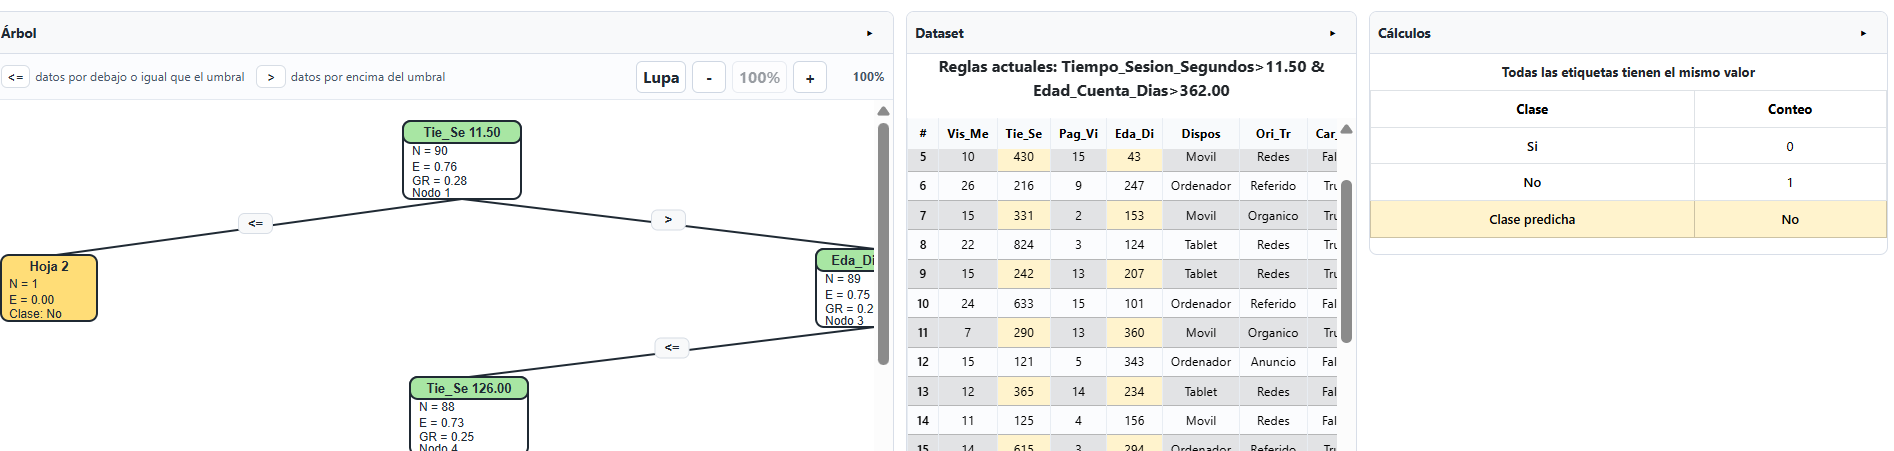
\includegraphics[width=0.75\textwidth]{img/Paneles_Expandidos.png}
     \caption{Paneles expandidos de la sección de simulación árbol C4.5.}
     \label{Fig_5.3}
 \end{figure}

 \begin{figure}[htbp]
     \centering
     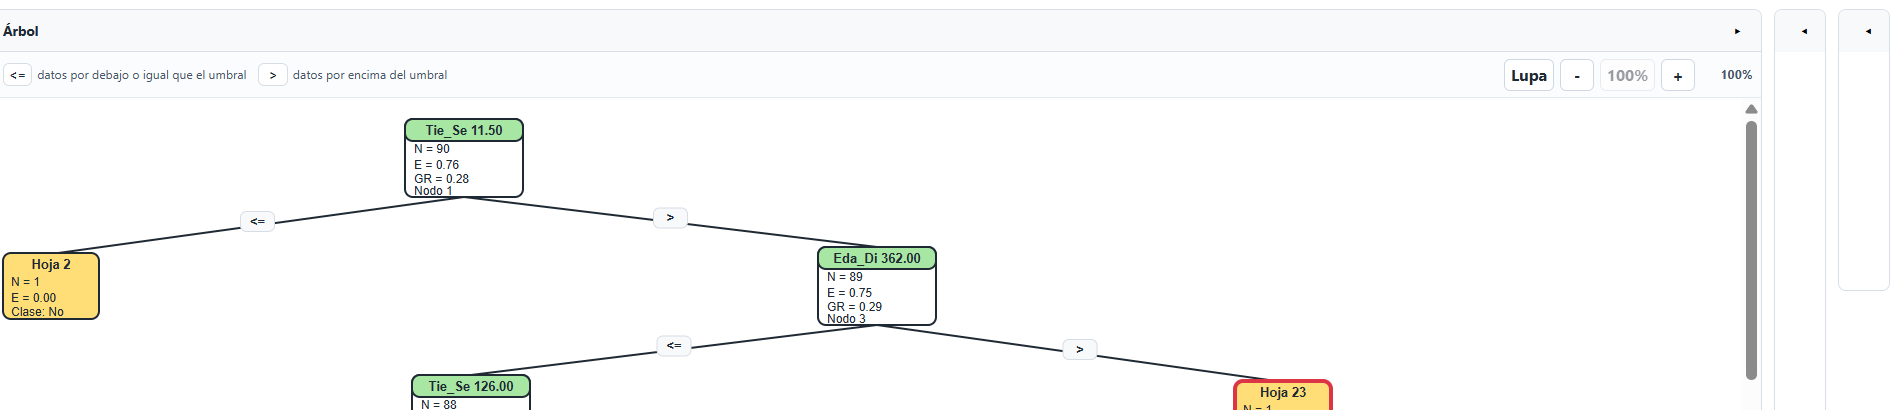
\includegraphics[width=0.75\textwidth]{img/Paneles_Contraidos.png}
     \caption{Paneles contraídos de la sección de simulación árbol C4.5.}
     \label{Fig_5.4}
 \end{figure}

\section{Visualización de árboles de gran tamaño}

Uno de los principales problemas encontrados durante el desarrollo fue la visualización de árboles de decisión de gran tamaño. A medida que aumenta el número de nodos y hojas, la representación gráfica puede ocupar un espacio considerable y dificultar la lectura de los valores mostrados en cada elemento.

Para facilitar la consulta del árbol, se incorporó una función de \textit{zoom} dentro del panel de visualización. Esta funcionalidad permite ampliar la representación del árbol y observar con mayor claridad los nodos, hojas y conexiones generadas durante cada paso de la simulación. En las figuras \ref{Fig_5.5} y \ref{Fig_5.6}, se muestran dos ejemplos del uso del \textit{zoom} en el panel del árbol.

Además, se añadió una herramienta de lupa que amplía la zona situada bajo el cursor del ratón. De este modo, el usuario puede consultar partes concretas del árbol sin tener que modificar continuamente el nivel de \textit{zoom} general de la representación. En la figura \ref{Fig_5.7} se muestra un ejemplo de uso de la lupa en el árbol

También se aplicaron medidas para mejorar la legibilidad de los nombres asociados a los atributos. Cuando el nombre de una columna del conjunto de datos es demasiado largo, la aplicación lo acorta automáticamente para evitar que ocupe un espacio excesivo dentro de los nodos. No obstante, para evitar que esta reducción de texto genere ambigüedades, se añade un \textit{tooltip} que muestra el nombre completo del atributo al situar el cursor sobre el texto abreviado. En la figura \ref{Fig_5.8} se muestra un ejemplo de los nombres de columnas categóricas en árbol

En los nodos categóricos, las conexiones entre un nodo de decisión y sus nodos hijos muestran el valor de la categoría correspondiente sobre la línea de unión. Estos textos se distribuyen a lo largo de la conexión para reducir el riesgo de solapamiento. Asimismo, cuando el valor de una categoría debe abreviarse, se muestra su contenido completo mediante un \textit{tooltip}.

Estas decisiones permiten que los árboles de mayor tamaño mantengan una representación visual comprensible, incluso cuando contienen numerosas ramas, nodos y hojas.

\begin{figure}[htbp]
     \centering
     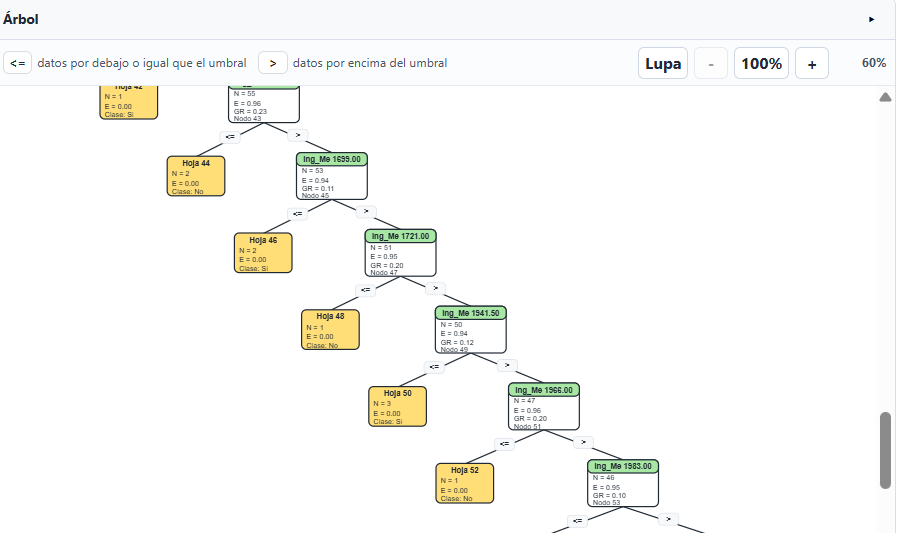
\includegraphics[width=0.75\textwidth]{img/Arbol_Sin_Zoom.png}
     \caption{Árbol sin \textit{zoom} en la sección de simulación árbol C4.5.}
     \label{Fig_5.5}
 \end{figure}

 \begin{figure}[htbp]
     \centering
     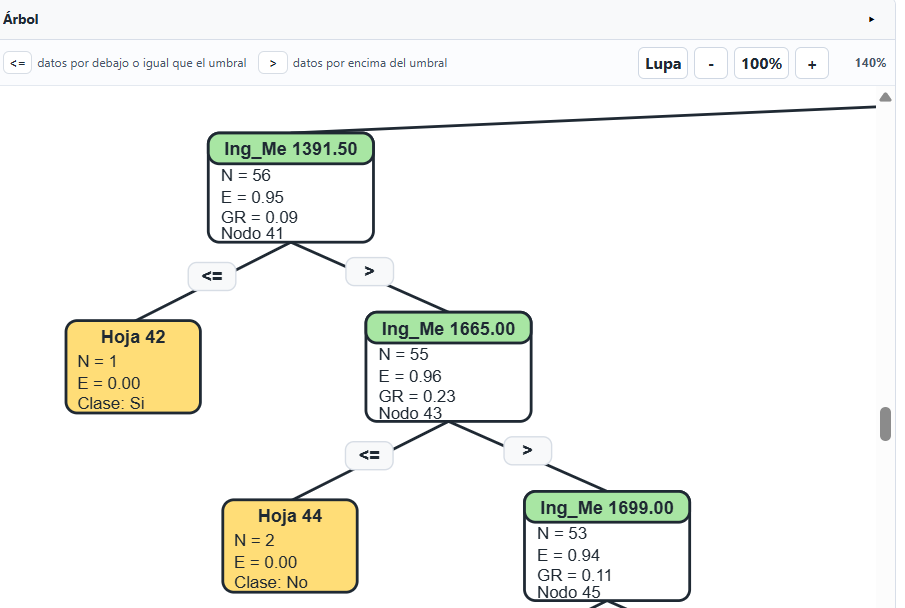
\includegraphics[width=0.75\textwidth]{img/Arbol_Con_Zoom.png}
     \caption{Árbol con \textit{zoom} en la sección de simulación árbol C4.5.}
     \label{Fig_5.6}
 \end{figure}

 \begin{figure}[htbp]
     \centering
     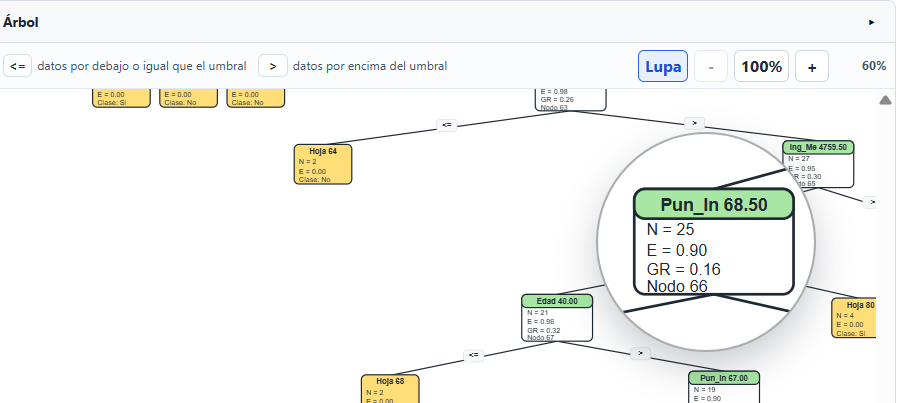
\includegraphics[width=0.75\textwidth]{img/Arbol_Lupa.png}
     \caption{Lupa del árbol en la sección de simulación árbol C4.5.}
     \label{Fig_5.7}
 \end{figure}

 \begin{figure}[htbp]
     \centering
     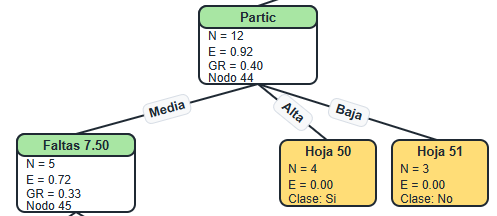
\includegraphics[width=0.75\textwidth]{img/Nombres_Columnas_Categoricas.png}
     \caption{Visualización de las categorías en las columnas en la sección de simulación árbol C4.5.}
     \label{Fig_5.8}
 \end{figure}

\section{Seguimiento del nodo generado en cada iteración}

La generación de árboles de decisión puede resultar difícil de seguir cuando el árbol contiene numerosos niveles. En estos casos, el usuario puede perder la referencia sobre el nodo que se está evaluando o sobre la hoja que acaba de crearse durante una iteración concreta.

Para evitar esta situación, se implementó un mecanismo de seguimiento automático del último elemento generado. Cada vez que la simulación crea un nuevo nodo o una nueva hoja, el árbol se centra automáticamente sobre dicho elemento y lo resalta visualmente.

De esta forma, el usuario puede identificar de manera inmediata qué parte de la estructura ha sido modificada en el paso actual. Esta decisión facilita el seguimiento de la simulación y permite relacionar los cálculos mostrados en el panel correspondiente con el nodo o la hoja que se está generando en el árbol.

La funcionalidad resulta especialmente útil en árboles de gran tamaño, en los que una nueva rama puede quedar fuera de la zona visible si el usuario se encuentra observando otra parte de la representación. En la figura \ref{Fig_5.9} se muestra como se remarca la hoja el seguimiento de los pasos del árbol.

\begin{figure}[htbp]
     \centering
     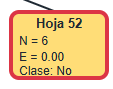
\includegraphics[width=0.2\textwidth]{img/Hoja_Paso.png}
     \caption{Visualización del remarque de la hoja en la sección de simulación árbol C4.5.}
     \label{Fig_5.9}
 \end{figure}

\section{Separación entre la construcción y la poda del árbol}

Uno de los aspectos más complejos del desarrollo fue la incorporación del proceso de poda. Aunque la poda forma parte del algoritmo C4.5, su funcionamiento requiere cálculos específicos y un procedimiento independiente de la construcción inicial del árbol.

En la fase de construcción, la simulación se centra en seleccionar el atributo o umbral más adecuado para dividir los datos y crear nuevos nodos hasta alcanzar las condiciones de parada. En cambio, la poda analiza posteriormente determinados nodos internos para decidir si conviene mantener el subárbol generado o sustituirlo por una hoja.

Debido a esta diferencia conceptual y operativa, se decidió segmentar la simulación en dos secciones diferenciadas. La primera sección muestra paso a paso la construcción del árbol de decisión. La segunda sección se dedica exclusivamente al proceso de poda y permite analizar cómo se evalúan los nodos candidatos. En la figura \ref{Fig_5.10} se muestra la división de los apartados

\begin{figure}[htbp]
     \centering
     
\includegraphics[width=0.75\textwidth]{img/Division_Poda_Arbol.png}
     \caption{Visualización de la separación entre la poda y la simulación árbol C4.5.}
     \label{Fig_5.10}
 \end{figure}

Ambas secciones mantienen una estructura visual similar, con paneles destinados al árbol, los datos y los cálculos correspondientes. Sin embargo, en la simulación de poda se incorpora información específica sobre el nodo que está siendo evaluado, los errores estimados del subárbol y de la hoja alternativa, así como la conclusión final sobre si el subárbol debe mantenerse o sustituirse por una hoja. En las figuras \ref{Fig_5.11} y \ref{Fig_5.12} se muestran los datos que aparecen en el panel de cálculos de la poda, visualizados el nodo evaluado y los cálculos para determinar la poda del mismo.

\begin{figure}[htbp]
     \centering
     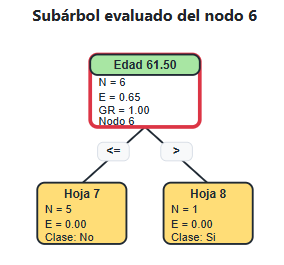
\includegraphics[width=0.5\textwidth]{img/SVG_Poda_Calculo.png}
     \caption{Visualización del nodo evaluado en el panel de cálculos de la poda}
     \label{Fig_5.11}
 \end{figure}

 \begin{figure}[htbp]
     \centering
     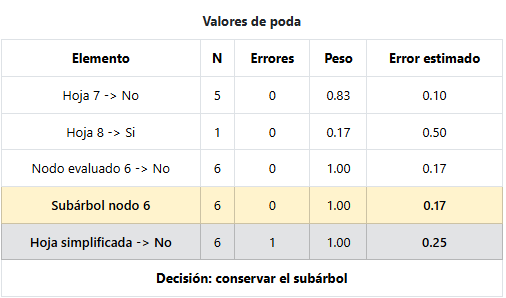
\includegraphics[width=0.75\textwidth]{img/Valores_Calculo_Poda.png}
     \caption{Visualización de los cálculos del nodo evaluado en el panel de cálculos de la poda}
     \label{Fig_5.12}
 \end{figure}

Asimismo, se añadieron \textit{tooltips} en el panel de cálculos de poda para explicar el origen de los valores utilizados. Esta ayuda adicional resulta necesaria porque la poda incluye cálculos diferentes a los utilizados durante la construcción del árbol y no se explican en las secciones teóricas generales de selección de atributos.

La división de la simulación en estas dos partes permite presentar el algoritmo de forma más ordenada y evita que la complejidad de la poda interfiera en la comprensión del proceso inicial de construcción del árbol.

\section{Selección del criterio de división}

Durante las fases finales del desarrollo se identificó una diferencia entre el criterio utilizado habitualmente en la docencia y el criterio propio del algoritmo C4.5. En determinados contextos educativos, el proceso de selección de atributos se explica utilizando la ganancia de información como valor principal. Sin embargo, C4.5 utiliza el \textit{gain ratio} como criterio de selección, con el objetivo de reducir el sesgo que puede producirse hacia atributos con un número elevado de valores distintos.

Esta diferencia podía provocar que el árbol mostrado por la aplicación no coincidiera con el que los estudiantes esperaban obtener durante la resolución manual de ejercicios explicados en clase. Por este motivo, se decidió incorporar una opción adicional en la ventana modal utilizada para cargar un archivo CSV.

Esta opción permite al usuario seleccionar si desea visualizar la construcción del árbol tomando como referencia la ganancia de información o el \textit{gain ratio}. La modalidad basada en la ganancia de información se ha incorporado con una finalidad didáctica, ya que permite adaptar la simulación a determinados ejemplos utilizados en el aula. En la figura \ref{Fig_5.13} se muestra la elección entre ganancia de información y \textit{gain ratio}.

\begin{figure}[htbp]
     \centering
     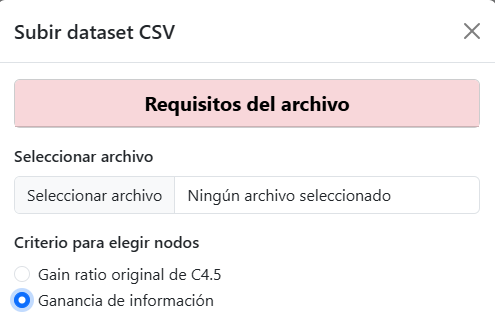
\includegraphics[width=0.75\textwidth]{img/GainRatio_Ganancia.png}
     \caption{Visualización la elección entre ganancia de información y \textit{gain ratio}}
     \label{Fig_5.13}
 \end{figure}

No obstante, la aplicación informa al usuario de que el criterio de selección característico del algoritmo C4.5 es el \textit{gain ratio}. De este modo, se mantiene la fidelidad respecto al funcionamiento del algoritmo y, al mismo tiempo, se proporciona flexibilidad para adaptar la herramienta a distintos enfoques docentes. En la figura \ref{Fig_5.14} se muestra el aviso que informa al usuario de que, aunque en la simulación se utiliza la ganancia de información como criterio de elección, el algoritmo C4.5 emplea el \textit{gain ratio} como criterio de decisión.

\begin{figure}[htbp]
     \centering
     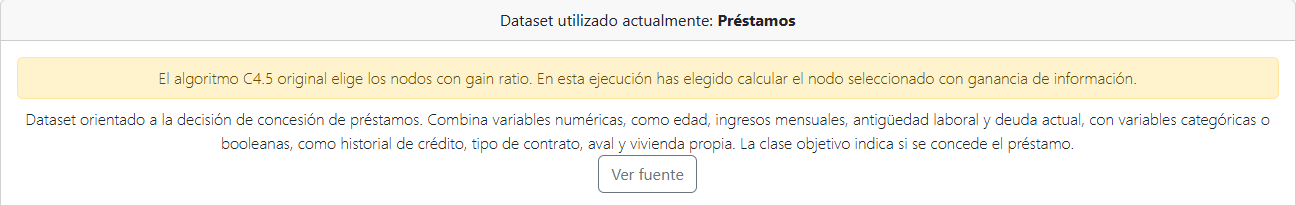
\includegraphics[width=0.75\textwidth]{img/Aviso_GainRatio.png}
     \caption{Visualización del aviso al usuario}
     \label{Fig_5.14}
 \end{figure}

\section{Validación y limitaciones de los archivos CSV}

La posibilidad de cargar conjuntos de datos propios constituye una de las funcionalidades más relevantes de la aplicación. Esta característica permite al usuario utilizar conjuntos de datos obtenidos de fuentes externas o creados por él mismo para observar cómo cambian los cálculos y la estructura final del árbol.

Sin embargo, la carga de archivos personalizados también exige establecer restricciones para evitar errores de procesamiento, problemas de visualización o conjuntos de datos incompatibles con la versión actual de la simulación.

Por este motivo, se implementó una validación previa de los archivos CSV antes de iniciar la construcción del árbol. Los requisitos establecidos para los conjuntos de datos son los siguientes:

\begin{itemize}
    \item El archivo debe estar en formato CSV y utilizar la coma como separador de valores.
    
    \item La primera fila debe contener los nombres de los atributos o cabeceras de las columnas.
    
    \item El conjunto de datos no puede contener más de 150 filas de datos.
    
    \item El archivo no puede contener más de 25 columnas.
    
    \item La cabecera no puede contener columnas vacías.
    
    \item Todas las filas deben contener el mismo número de columnas.
    
    \item No se permiten valores vacíos dentro del conjunto de datos.
    
    \item Todos los valores de una misma columna deben pertenecer al mismo tipo de dato.
    
    \item Los formatos de datos admitidos son numéricos, booleanos y categóricos.
    
    \item La última columna debe corresponder a la clase objetivo que se desea predecir.
    
    \item La columna de clase debe contener exactamente dos valores distintos.
\end{itemize}

La limitación de 150 filas y 25 columnas se estableció principalmente para mantener una experiencia de uso adecuada. Un conjunto de datos demasiado grande puede generar árboles extensos y difíciles de interpretar, reduciendo el valor didáctico de la aplicación.

Asimismo, aunque el algoritmo C4.5 puede utilizarse en problemas con más de dos clases, la versión actual de la herramienta limita la clase objetivo a dos valores distintos. Esta restricción permite simplificar la visualización, los cálculos y la explicación del proceso de construcción del árbol dentro del alcance definido para el proyecto.

Las validaciones implementadas permiten informar al usuario cuando un archivo no cumple las condiciones necesarias y evitan que se intente ejecutar el algoritmo sobre conjuntos de datos incompletos, inconsistentes o demasiado grandes para su correcta representación en la interfaz.

